\documentclass{standalone}
\usepackage{tikz}
\usetikzlibrary{patterns}
\usetikzlibrary{positioning}
\usetikzlibrary{patterns, positioning}
\usetikzlibrary{shapes.misc}
\usepackage[outline]{contour}
\contourlength{1.5pt} 
\usepackage[sfdefault]{ClearSans}

\begin{document}
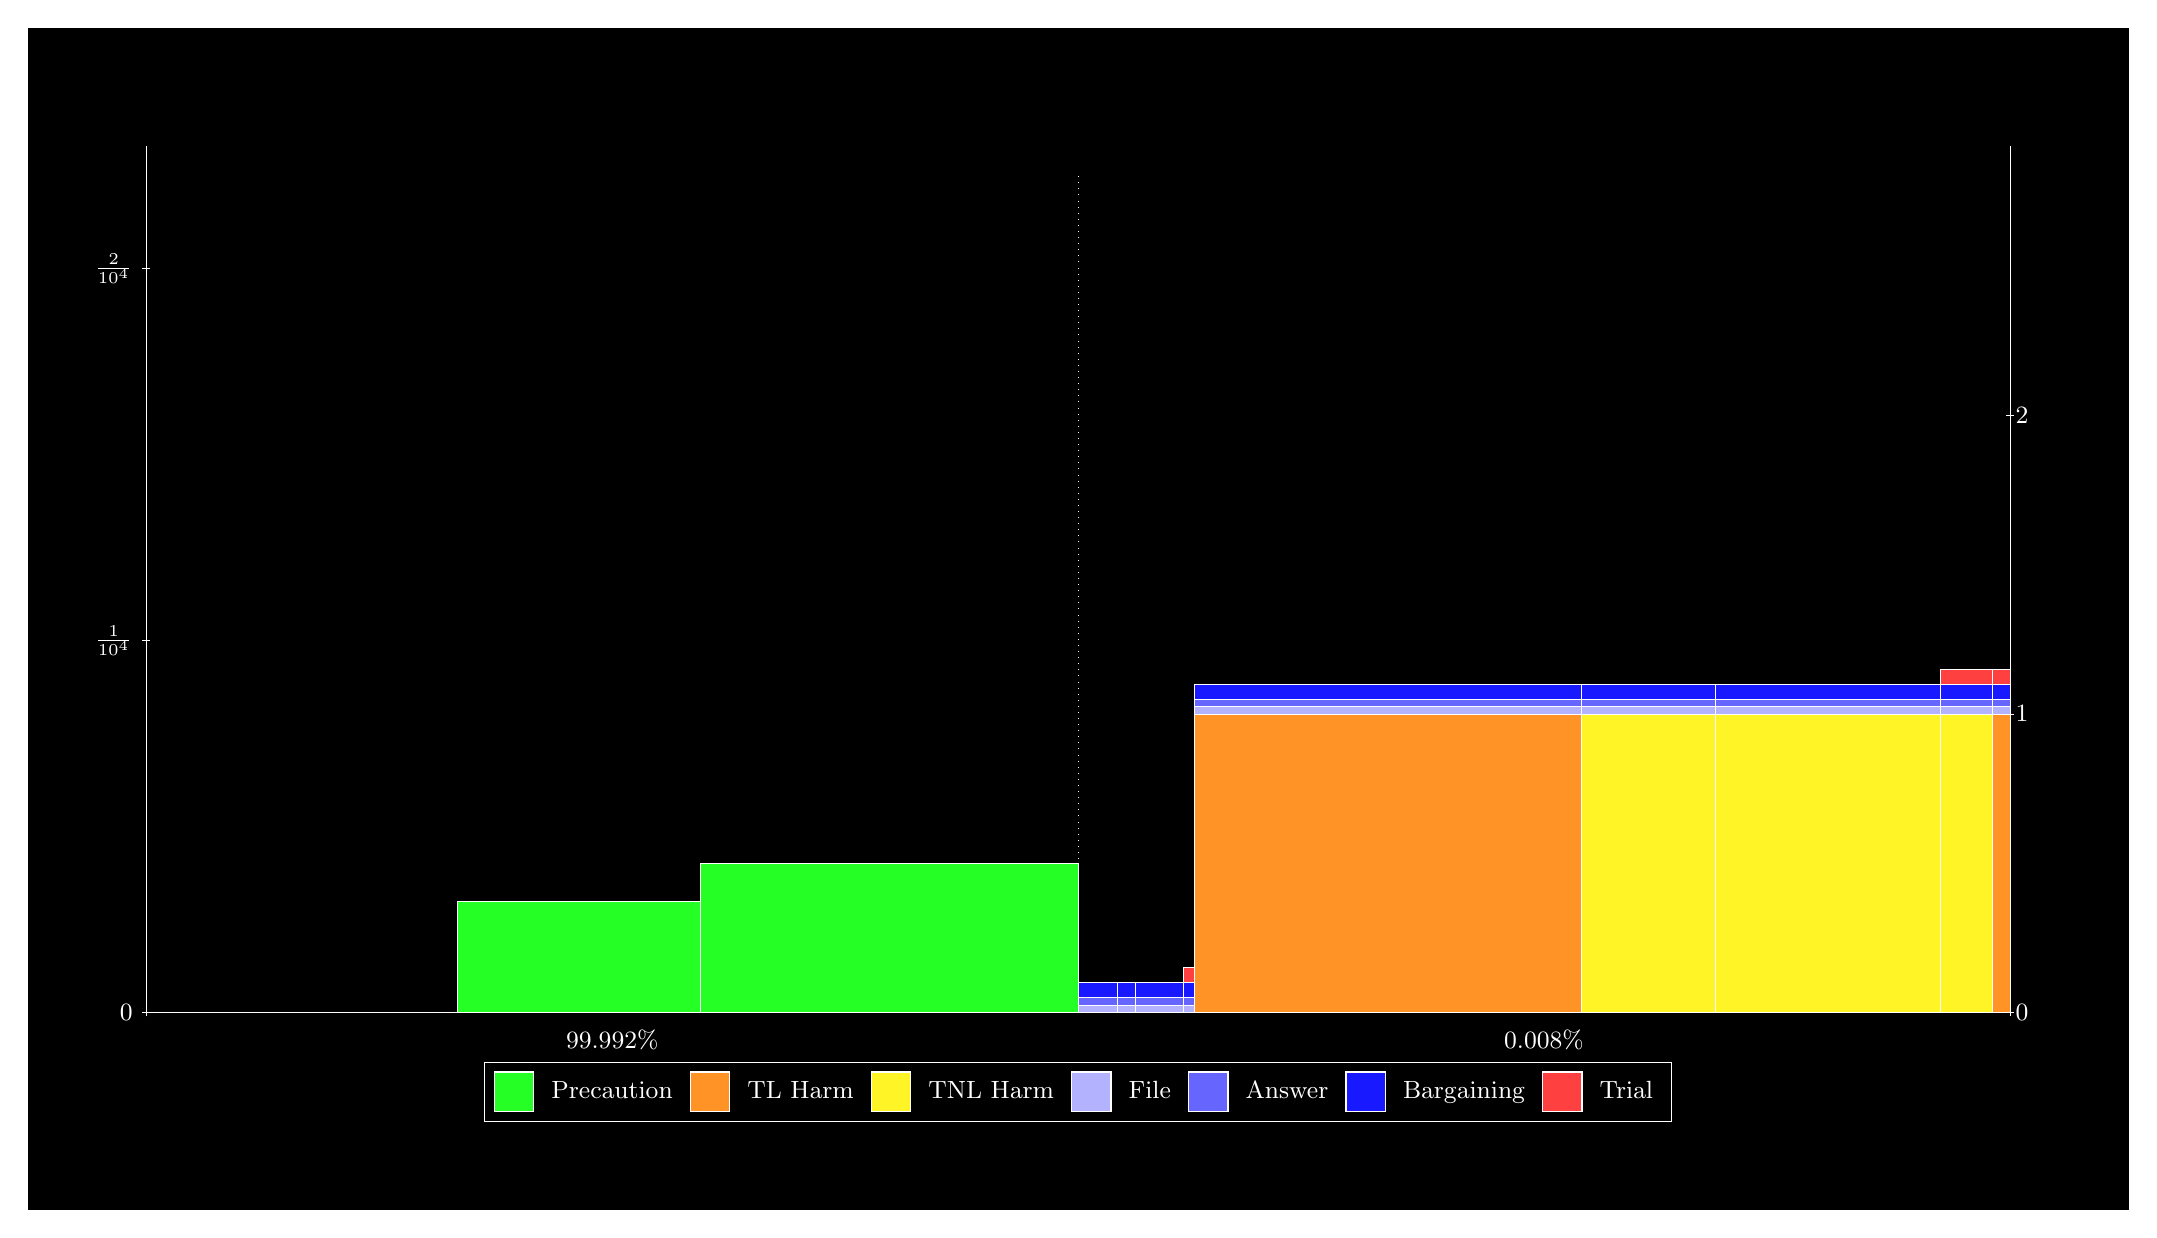
\begin{tikzpicture}
\draw[fill=black] (0,0) rectangle (26.667,15);
\draw[fill=green!85,draw=white,very thin] (5.4443,2.5) rectangle (8.538,3.9173);
\draw[fill=green!85,draw=white,very thin] (8.538,2.5) rectangle (13.333,4.3897);
\draw[fill=blue!30,draw=white,very thin] (13.333,2.5) rectangle (13.825,2.5948);
\draw[fill=blue!60,draw=white,very thin] (13.333,2.5948) rectangle (13.825,2.6896);
\draw[fill=blue!90,draw=white,very thin] (13.333,2.6896) rectangle (13.825,2.8791);
\draw[fill=green!85,draw=white,very thin] (13.825,2.5) rectangle (14.065,2.5001);
\draw[fill=blue!30,draw=white,very thin] (13.825,2.5001) rectangle (14.065,2.5949);
\draw[fill=blue!60,draw=white,very thin] (13.825,2.5949) rectangle (14.065,2.6897);
\draw[fill=blue!90,draw=white,very thin] (13.825,2.6897) rectangle (14.065,2.8792);
\draw[fill=green!85,draw=white,very thin] (14.065,2.5) rectangle (14.663,2.5002);
\draw[fill=blue!30,draw=white,very thin] (14.065,2.5002) rectangle (14.663,2.5949);
\draw[fill=blue!60,draw=white,very thin] (14.065,2.5949) rectangle (14.663,2.6897);
\draw[fill=blue!90,draw=white,very thin] (14.065,2.6897) rectangle (14.663,2.8793);
\draw[fill=green!85,draw=white,very thin] (14.663,2.5) rectangle (14.808,2.5001);
\draw[fill=blue!30,draw=white,very thin] (14.663,2.5001) rectangle (14.808,2.5949);
\draw[fill=blue!60,draw=white,very thin] (14.663,2.5949) rectangle (14.808,2.6897);
\draw[fill=blue!90,draw=white,very thin] (14.663,2.6897) rectangle (14.808,2.8792);
\draw[fill=red!75,draw=white,very thin] (14.663,2.8792) rectangle (14.808,3.0688);
\draw[fill=orange!85,draw=white,very thin] (14.808,2.5) rectangle (19.723,6.2913);
\draw[fill=blue!30,draw=white,very thin] (14.808,6.2913) rectangle (19.723,6.3861);
\draw[fill=blue!60,draw=white,very thin] (14.808,6.3861) rectangle (19.723,6.4809);
\draw[fill=blue!90,draw=white,very thin] (14.808,6.4809) rectangle (19.723,6.6705);
\draw[fill=green!85,draw=white,very thin] (19.723,2.5) rectangle (21.419,2.5001);
\draw[fill=yellow!85,draw=white,very thin] (19.723,2.5001) rectangle (21.419,6.2915);
\draw[fill=blue!30,draw=white,very thin] (19.723,6.2915) rectangle (21.419,6.3862);
\draw[fill=blue!60,draw=white,very thin] (19.723,6.3862) rectangle (21.419,6.481);
\draw[fill=blue!90,draw=white,very thin] (19.723,6.481) rectangle (21.419,6.6706);
\draw[fill=green!85,draw=white,very thin] (21.419,2.5) rectangle (21.431,2.5001);
\draw[fill=orange!85,draw=white,very thin] (21.419,2.5001) rectangle (21.431,6.2915);
\draw[fill=blue!30,draw=white,very thin] (21.419,6.2915) rectangle (21.431,6.3862);
\draw[fill=blue!60,draw=white,very thin] (21.419,6.3862) rectangle (21.431,6.481);
\draw[fill=blue!90,draw=white,very thin] (21.419,6.481) rectangle (21.431,6.6706);
\draw[fill=green!85,draw=white,very thin] (21.431,2.5) rectangle (24.28,2.5002);
\draw[fill=yellow!85,draw=white,very thin] (21.431,2.5002) rectangle (24.28,6.2915);
\draw[fill=blue!30,draw=white,very thin] (21.431,6.2915) rectangle (24.28,6.3863);
\draw[fill=blue!60,draw=white,very thin] (21.431,6.3863) rectangle (24.28,6.4811);
\draw[fill=blue!90,draw=white,very thin] (21.431,6.4811) rectangle (24.28,6.6706);
\draw[fill=green!85,draw=white,very thin] (24.28,2.5) rectangle (24.941,2.5001);
\draw[fill=yellow!85,draw=white,very thin] (24.28,2.5001) rectangle (24.941,6.2915);
\draw[fill=blue!30,draw=white,very thin] (24.28,6.2915) rectangle (24.941,6.3862);
\draw[fill=blue!60,draw=white,very thin] (24.28,6.3862) rectangle (24.941,6.481);
\draw[fill=blue!90,draw=white,very thin] (24.28,6.481) rectangle (24.941,6.6706);
\draw[fill=red!75,draw=white,very thin] (24.28,6.6706) rectangle (24.941,6.8602);
\draw[fill=green!85,draw=white,very thin] (24.941,2.5) rectangle (25.167,2.5001);
\draw[fill=orange!85,draw=white,very thin] (24.941,2.5001) rectangle (25.167,6.2915);
\draw[fill=blue!30,draw=white,very thin] (24.941,6.2915) rectangle (25.167,6.3862);
\draw[fill=blue!60,draw=white,very thin] (24.941,6.3862) rectangle (25.167,6.481);
\draw[fill=blue!90,draw=white,very thin] (24.941,6.481) rectangle (25.167,6.6706);
\draw[fill=red!75,draw=white,very thin] (24.941,6.6706) rectangle (25.167,6.8602);
\draw[white,very thin] (1.5,2.5) -- (1.5,13.5);
\draw[white,very thin] (1.45,2.5) -- (1.55,2.5);
\node[font=\small,text=white, anchor=east] at (1.45, 2.5) {0};
\draw[white,very thin] (1.45,7.2243) -- (1.55,7.2243);
\node[font=\small,text=white, anchor=east] at (1.45, 7.2243) {$\frac{1}{10^{4}}$};
\draw[white,very thin] (1.45,11.949) -- (1.55,11.949);
\node[font=\small,text=white, anchor=east] at (1.45, 11.949) {$\frac{2}{10^{4}}$};

\draw[white,dotted,very thin] (13.333,2.83) -- (13.333,13.17);
\draw[white,very thin] (25.167,2.5) -- (25.167,13.5);
\draw[white,very thin] (25.117,2.5) -- (25.217,2.5);
\node[font=\small,text=white, anchor=west] at (25.117, 2.5) {0};
\draw[white,very thin] (25.117,6.2913) -- (25.217,6.2913);
\node[font=\small,text=white, anchor=west] at (25.117, 6.2913) {1};
\draw[white,very thin] (25.117,10.083) -- (25.217,10.083);
\node[font=\small,text=white, anchor=west] at (25.117, 10.083) {2};

\draw[white,very thin] (1.5,2.5) -- (25.167,2.5);
\draw[white,very thin] (1.5,2.45) -- (1.5,2.55);
\node[font=\small,text=white, anchor=north] at (1.5, 2.45) {};
\draw[white,very thin] (25.167,2.45) -- (25.167,2.55);
\node[font=\small,text=white, anchor=north] at (25.167, 2.45) {};

\node[font=\small,text=white,anchor=south] at (7.4167, 1.9) {99.992\%};
\node[font=\small,text=white,anchor=south] at (19.25, 1.9) {0.008\%};
\draw (13.3333,2.5) node (B) {};
\begin{scope}[align=center]
\matrix[scale=0.5,draw=white,below=0.5cm of B,nodes={draw},column sep=0.1cm]{
\node[rectangle,draw,minimum width=0.5cm,minimum height=0.5cm,fill=green!85]{}; & \node[draw=none,font=\small,text=white]{Precaution}; &
\node[rectangle,draw,minimum width=0.5cm,minimum height=0.5cm,fill=orange!85]{}; & \node[draw=none,font=\small,text=white]{TL Harm}; &
\node[rectangle,draw,minimum width=0.5cm,minimum height=0.5cm,fill=yellow!85]{}; & \node[draw=none,font=\small,text=white]{TNL Harm}; &
\node[rectangle,draw,minimum width=0.5cm,minimum height=0.5cm,fill=blue!30]{}; & \node[draw=none,font=\small,text=white]{File}; &
\node[rectangle,draw,minimum width=0.5cm,minimum height=0.5cm,fill=blue!60]{}; & \node[draw=none,font=\small,text=white]{Answer}; &
\node[rectangle,draw,minimum width=0.5cm,minimum height=0.5cm,fill=blue!90]{}; & \node[draw=none,font=\small,text=white]{Bargaining}; &
\node[rectangle,draw,minimum width=0.5cm,minimum height=0.5cm,fill=red!75]{}; & \node[draw=none,font=\small,text=white]{Trial}; \\\\
};\end{scope}

\end{tikzpicture}
\end{document}